\chapter[Escolha GPS]{Escolha Sistema de Posicionamento Global}

\section{Aspectos Gerais}

O Sistema de Posicionamento Global, GPS, é um sistema de radionavegação
baseado em satélite, que foi desenvolvido na década de 70, pelo departamento
de Defesa dos Estados Unidos e pode ser dividido em três segmentos principais:
segmento espacial, segmento de controle e segmento de usuário \cite{interferidores_gps}.
Como ilustrado na figura 01, o segmento espacial é constituído por
24 satélites, dispostos em 6 planos orbitais e igualmente espaçados,
permitindo que a qualquer momento, pelo menos 4 satélites, tenha
comunicação com o receptor. O sistema de controle monitora e corrige
relógios, além de atualizar as mensagens de navegação de cada satélite,
este segmento possui 5 estações terrestres. Já o terceiro segmento é
constituído pelos receptores GPS \cite{posicionamento_gnss}.

\begin{figure}[h]
  \centering
  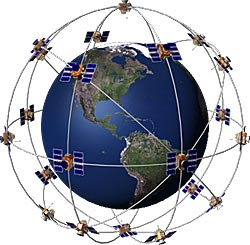
\includegraphics[width=200px, scale=1]{figuras/esquema_gps}
  \caption{Segmento Espacial do sistema GPS \cite{entendendo_gps}}
\label{fig:esquema_gps}
\end{figure}

O sistema GPS oferece aos usuários, informação exata, continua e
tridimensional de posição e velocidade de maneira ilimitada, uma
vez que os usuários atuam de forma passiva. Para determinar a posição
do usuário, o sistema utiliza o conceito one-way time arrivel, TOA, que
mede o tempo que o sinal transmitido por um emissor em um local conhecido,
leva para chegar ao receptor, multiplica o de tempo pela velocidade de
propagação do sinal e assim obtém a distância emissor-receptor \cite{sobre_gps}.

Tendo em vista que o sistema proposto com este projeto visa calcular e
identificar quando há ou não a possibilidade de ultrapassagem, o sistema
GPS é necessário para identificar a posição dos veículos quando há a
intenção de ultrapassagem, já que, como citado anteriormente, em qualquer
ponto da terra, pelo menos 4 satélites conseguem identificar a posição do
usuário, além disso não há necessidade de intervisibilidade entre estações
para seu funcionamento e ele opera sob quaisquer condições climáticas \cite{sobre_gps}.

\section{Especificações do GPS}

O GPS possui dois modos de operação, o padrão, Standard Positioning Service,
SPS, e o preciso, Precise Positioning Service, PPS. O SPS é gratuito e tem
precisão de 120 a 140 m e de 10 a 20 m, enquanto o PPS, é de uso restrito
militar e apresenta precisão de 10 a 20 m. O SPS tem precisão limitada e
seletiva imposta pelo Departamento de Defesa Americano, por um processo de
criptografia aplicado em um dos códigos do sistema que torna as medições
menos precisas se necessário \cite{6gps}.

Os satélites transmitem continuamente um sinal de rádio com informações sobre
a sua posição orbital e tempo marcado por seu relógio atômico interno \cite{7gps}.
 Esse sinal eletromagnético é chamado de onda portadora e passa por um
 procedimento de modulação antes de ser irradiado pelo espaço, esse processo
 de modulação consiste em modificar um sinal eletromagnético de forma que
 transporte informações, como dados de posição e tempo \cite{8gps}.

O sistema receptor armazena o tempo medido e os valores de tempo registrados
pelos satélites no momento do envio da onda portadora, com base nesse dado e
 na velocidade de propagação das ondas, que é conhecida, através da equação
 a seguir se obtém a distância \cite{8gps}.

 $ \Delta S = V \times  \Delta t $

 Onde:

 $ \Delta S $ é a distância entre o satélite e o receptor.
V é a velocidade de propagação da onda.

$ \Delta t $ é o tempo de envio da onda portadora.

Como citado na seção 1.1, o GPS possui três segmentos, espacial, de controle e
de usuário, a figura \ref{fig:segmentos_gps} ilustra a iteração dos segmentos.


\begin{figure}[h]
  \centering
  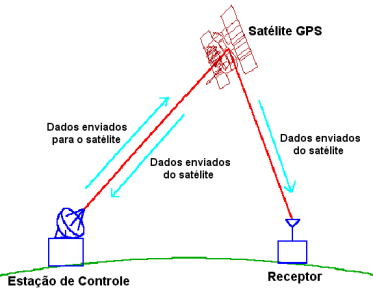
\includegraphics[width=250px, scale=1]{figuras/segmentos_gps}
  \caption{Segmentos de GPS  \cite{9gps}}
\label{fig:segmentos_gps}
\end{figure}


\section{JUSTIFICATIVAS DE ESCOLHA}
\subsection{GPS A2100-A/B}

Esse módulo faz a aquisição e rastreamento de forma rápida e tem aplicação
 para consumidores móveis. Além disso o módulo tem boa sensibilidade e pode
 ser utilizado em muitos ambientes diferentes, sob condições diversas \cite{10gps}.
 A tabela \ref{table:especificacao_gps23} mostra as especificações desse dispositivo e a figura \ref{fig:a2100} é a
 imagem do mesmo.


  \begin{table}[ht]
  \caption{Especificações do A2100-A/B. Baseado em: \cite{10gps}}
  \centering
  \begin{tabular}{| l |  p{4cm} |}
  \hline
  Característica & Valores \\
  \hline
  Canais & 48 \\
  \hline
  Frequência & 1,575 MHz \\
  \hline
  Precisão de distância & 2,5 m \\
  \hline
  Peso & 1,2 g \\
  \hline
  Dimensões L x A x P & 15,2 x 15,2 x 2,4 $ mm ^ {3} $ \\
  \hline
  Tensão de alimentação & 3,0 a 3,6 VDC \\
  \hline
  Alimentação da antena & Até 5,0 V \\
  \hline
  Corrente máxima da antena & 50 mA \\
  \hline
  Temperatura de operação & - 40ºC a +85 ºC \\
  \hline
  Sensibilidade de rastreamento & -163 dB \\
  \hline
  Sensibilidade de navegação & -160 dB \\
  \hline
  \end{tabular}
  \label{table:especificacao_gps23}
  \end{table}

  \begin{figure}[h]
    \centering
    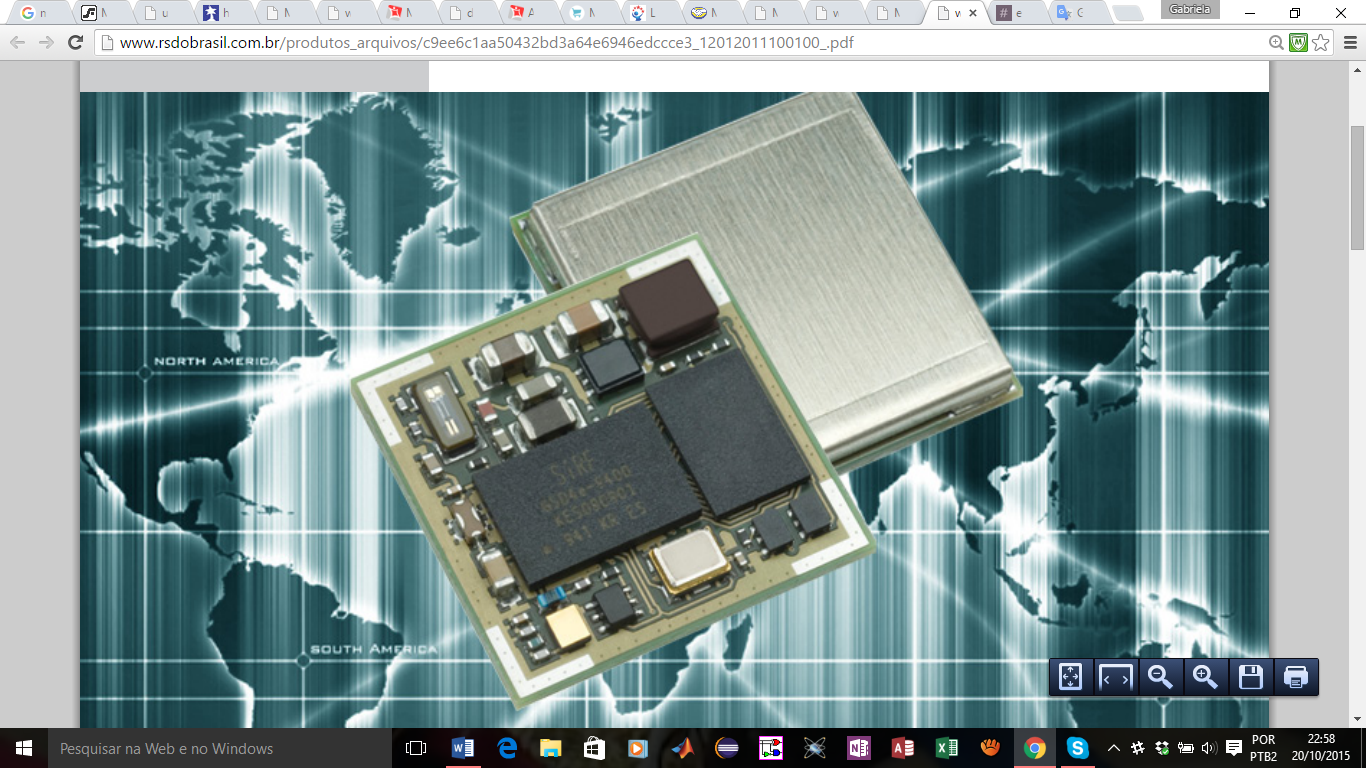
\includegraphics[width=200 px, scale=1]{figuras/a2100}
    \caption{A2100-A/B   \cite{10gps}}
  \label{fig:a2100}
  \end{figure}

  \subsection{ME-1000RW}

  O ME-1000RW é um módulo receptor GPS com antena acoplada. A antena é conectada
  ao receptor através de um Amplificador de Baixo Ruído. O receptor é capaz de
  receber sinais de até 65 satélites GPS e informar a posição e o tempo precisos,
  além disso possui baixo consumo \cite{11gps}. A figura \ref{fig:gps_me1000} e a tabela
  \ref{table:especificacao_gps_me1000}
  descrevem as  características do produto. O preço desse modulo é de R\$ 98,99 \cite{12gps}.


\begin{table}[ht]
\caption{Especificações do ME-1000RW Baseado em: \cite{11gps}}
\centering
\begin{tabular}{| l |  p{5cm} |}
\hline
Característica & Valores \\
\hline
Canais & 65 \\
\hline
Frequência & 1575,42 MHz \\
\hline
Precisão de distância & 5 m \\
\hline
Precisão de tempo & 300 ns \\
\hline
Precisão de velocidade & 0,1 m/s \\
\hline
Limite de operação para velocidade & 515 m/s \\
\hline
Peso & 28 g \\
\hline
Dimensões L x A x P & 32 x 32 x 8 mm \\
\hline
Tensão de operação & 3,6 a 6 VDC \\
\hline
Corrente máxima & 23 mA \\
\hline
Temperatura de operação & - 20ºC a +60ºC \\
\hline
Temperatura de armazenamento & -40ºC a +80ºC \\
\hline
Sensibilidade & -161 dB \\
\hline
\end{tabular}
\label{table:especificacao_gps_me1000}
\end{table}


\begin{figure}[h]
  \centering
  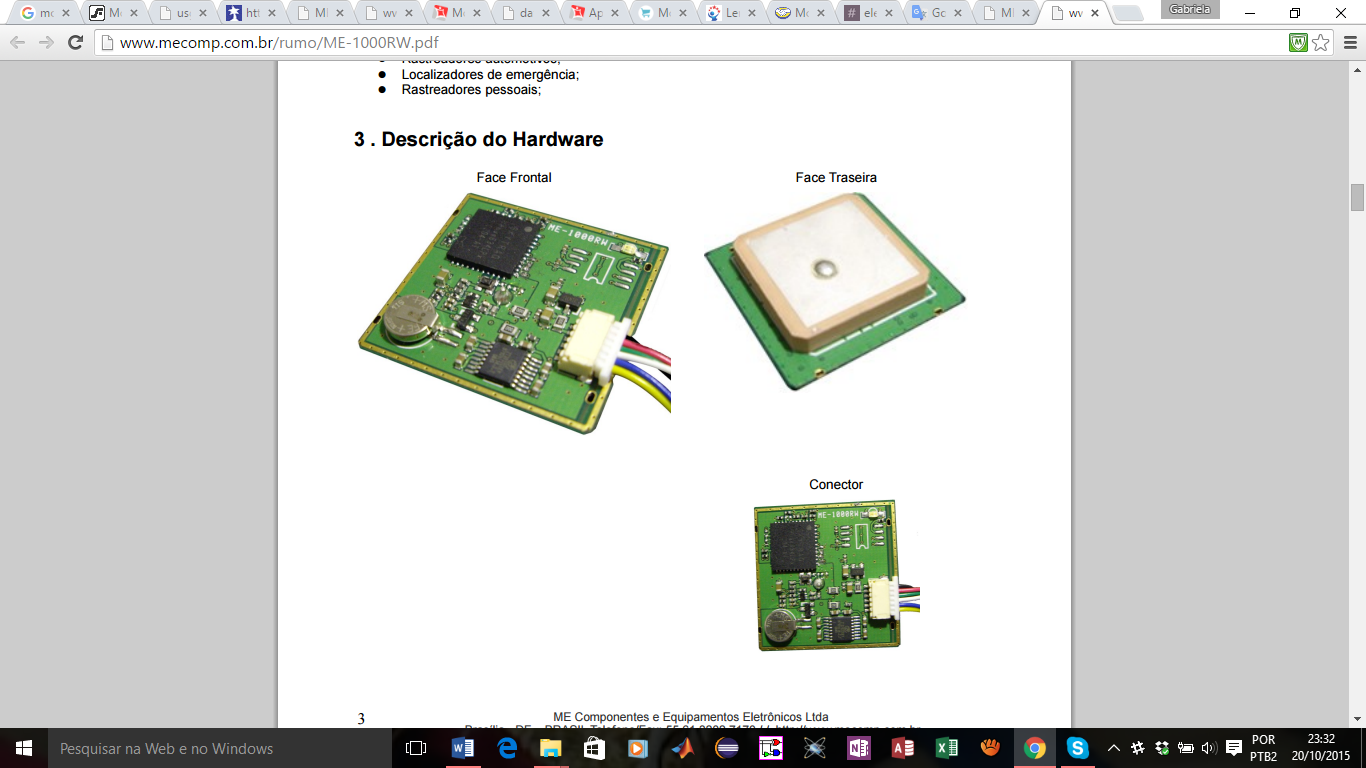
\includegraphics[width=200px, scale=1]{figuras/gps_me1000}
  \caption{ME-1000RW \cite{11gps}}
\label{fig:gps_me1000}
\end{figure}

\subsection{NEO - 6M}

O NEO-6M é um receptor de GPS autônomo, de alto desempenho, flexível e de
baixo custo, ideal para dispositivos móveis com restrições de custo e
 espaço. O dispositivo possui 50 canais e excelente performance de navegação,
 mesmo sob condições adversas \cite{13gps}. A tabela \ref{table:especificacao_gps_neo}
  e a figura \ref{fig:gps_neo}, ilustram as
 características desse modulo, que custa R\$88,20 \cite{14gps}.


 \begin{table}[ht]
 \caption{Especificações do NEO-6M Baseado em: \cite{13gps}}
 \centering
 \begin{tabular}{| l |  p{5cm} |}
 \hline
 Característica & Valores \\
 \hline
 Canais & 50 \\
 \hline
 Frequência & 1575,42 MHz \\
 \hline
 Precisão de distância & 2,5 m \\
 \hline
 Precisão de tempo & Precisão de velocidade \\
 \hline
 Limite de operação para velocidade & 500 m/s \\
 \hline
 Peso & 28 g \\
 \hline
 Dimensões L x A x P & 16 x 12,2 x 2,4 mm \\
 \hline
 Tensão de operação & 0,5 a 3,6 VDC \\
 \hline
 Tensão de operação & 0,5 a 3,6 VDC \\
 \hline
 Corrente máxima & 10 mA \\
 \hline
 Temperatura de operação & - 40ºC a +85ºC \\
 \hline
 Sensibilidade & -161 dB \\
 \hline
 \end{tabular}
 \label{table:especificacao_gps_neo}
 \end{table}

 \begin{figure}[h]
   \centering
   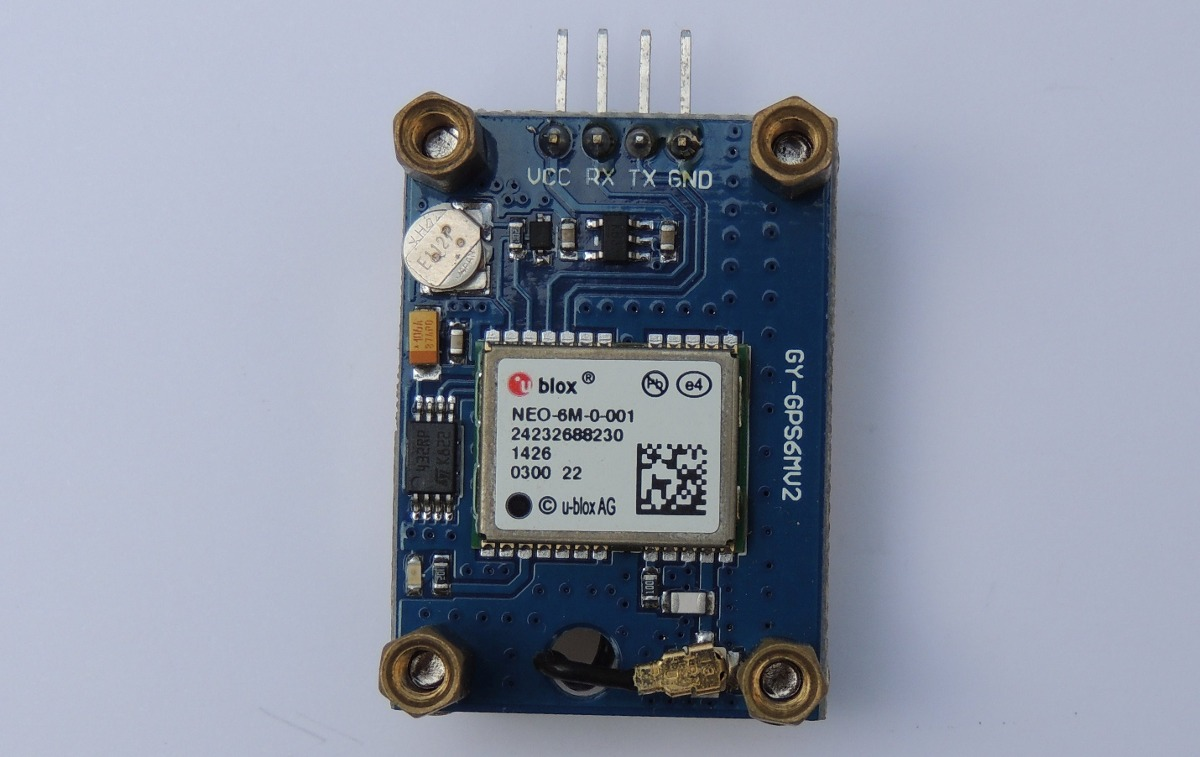
\includegraphics[width=200px, scale=1]{figuras/gps_neo}
   \caption{NEO-6M  \cite{14gps}}
 \label{fig:gps_neo}
 \end{figure}

 O módulo GPS A2200-A é a primeira implementação do Maestro de receptores
 GPS que podem ser usados altamente integrado como componentes SMT. Uma
 implementação muito fácil permite
 receber a posição, a velocidade e informação de tempo, é um módulo concebido
 para um ambiente de 3,3 V \cite{15gps}. Seu preço é R\$ 25,00 \cite{16gps}. Na tabela \ref{table:especificacao_gps_neo6m},
 estão as especificações do produto e a figura 06 é a imagem do mesmo.

 \begin{table}[ht]
 \caption{Especificações do NEO-6M. Baseado em: \cite{15gps}}
 \centering
 \begin{tabular}{| l |  p{5cm} |}
 \hline
 Característica & Valores \\
 \hline
 Canais & 48 \\
 \hline
 Frequência & 1,575 MHz \\
 \hline
 Precisão de distância & 2,5 m \\
 \hline
 Precisão de distância & 2,5 m \\
 \hline
 Precisão de tempo & Não informado \\
 \hline
 Precisão de velocidade & Não informado \\
 \hline
 Limite de operação para velocidade & Não informado \\
 \hline
 Peso & 0,6 g \\
 \hline
 Dimensões L x A x P & 14 x 10,2 x 2,5 mm \\
 \hline
 Tensão de operação & 3,0 a 3,6 VDC \\
 \hline
 Corrente máxima & 69 mA \\
 \hline
 Temperatura de operação & - 40ºC a +85ºC \\
 \hline
 Sensibilidade & -163 dB \\
 \hline
 \end{tabular}
 \label{table:especificacao_gps_neo6m}
 \end{table}

 \begin{figure}[h]
   \centering
   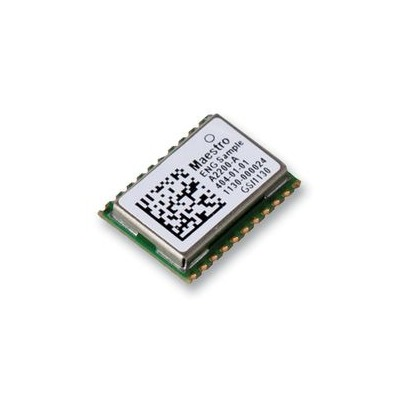
\includegraphics[width=200px, scale=1]{figuras/gps_neo_6m}
   \caption{NEO-6M 2200  \cite{16gps}}
 \label{fig:gps_neo_6m}
 \end{figure}

\section{CONCLUSÃO}

Foi constatado que os GPS têm valores de restrição muito parecidos, além de
estarem na mesma faixa de preço, com exceção do NEO-6M. Dessa forma o fator
decisivo para a escolha do módulo foi a interface serial. Conforme as
especificações do Transponder a ser utilizado no projeto, o módulo de GPS
  escolhido foi o ME-1000RW, que tem a mesma interface serial que o dispositivo.
